\subsubsection{UC19 - Abilitazione/disabilitazione account}
\begin{figure}[h]
	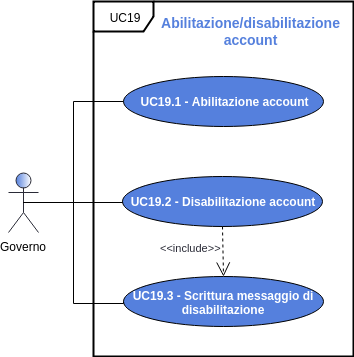
\includegraphics[width=8cm]{res/images/UC19.png}
	\centering
	\caption{UC19 - Abilitazione/disabilitazione account}
\end{figure}
\begin{itemize}
	\item \textbf{Attori Primari}:
	governo;
	\item \textbf{Descrizione}: il governo può gestire gli account degli utenti registrati alla piattaforma, in particolare può:
	\begin{itemize}
		\item abilitare un account;
		\item disabilitare un account, lasciando un messaggio relativo alla causa di tale provvedimento.
	\end{itemize}
	\item \textbf{Scenario principale}: il governo visualizza la lista degli utenti, aziende [UC18.1] o cittadini [UC18.4]. Per ognuna di esse ha la possibilità di abilitare l'account o disabilitarlo premendo l'apposito pulsante;
	\item \textbf{Precondizione}: l'utente governativo sta visualizzando una lista di utenti registrati al sistema, e può quindi accedere al pulsante per l'abilitazione o disabilitazione dell'account di un cittadino;
	\item \textbf{Postcondizione}: l'account dell'utente selezionato è stato abilitato o disabilitato. Nel caso sia stato disabilitato, durante i prossimi tentativi di autenticazione, tale utente riceverà l'errore di "account disabilitato" [UC8].
\end{itemize} 

\subsubsection{UC19.1 - Abilitazione account}
\begin{itemize}
	\item \textbf{Attori Primari}:
	governo;
	\item \textbf{Descrizione}: il governo può abilitare l'account di un utente;
	\item \textbf{Scenario principale}: il governo visualizza la lista degli utenti, aziende [UC18.1] o cittadini [UC18.4]. Per ogni utente il cui stato dell'account risulta "disabilitato", può effettuare l'abilitazione premendo sul pulsante dedicato;

	\item \textbf{Precondizione}: l'utente governativo sta visualizzando una lista di utenti registrati al sistema, preme il pulsante di abilitazione dell'account relativo ad un utente il quale stato dell'account risulta "disabilitato";
	\item \textbf{Postcondizione}: lo stato  dell'account utente sopra menzionato risulta "abilitato".
\end{itemize} 


\subsubsection{UC19.2 - Disabilitazione account}
\begin{figure}[h]
	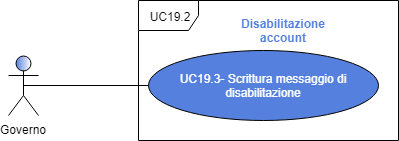
\includegraphics[width=8cm]{res/images/UC19-2.png}
	\centering
	\caption{UC19.2 - Disabilitazione account}
\end{figure}
\begin{itemize}
	\item \textbf{Attori Primari}:
	governo;
	\item \textbf{Descrizione}: il governo può disabilitare l'account di un utente;
	\item \textbf{Scenario principale}: il governo visualizza la lista degli utenti, aziende [UC18.1] o cittadini [UC18.4]. Per ogni utente il cui stato dell'account risulta "abilitato", può effettuare la disabilitazione premendo sul pulsante dedicato;
	\item \textbf{Inclusioni}: 
	\begin{itemize}
		\item \textbf{UC19.3}: durante la disabilitazione l'utente governativo è richiesto di inserire un messaggio personalizzato per spiegare all'utente il motivo della disabilitazione dell'account.
	\end{itemize}
	\item \textbf{Precondizione}: l'utente governativo sta visualizzando una lista di utenti registrati al sistema, preme il pulsante di disabilitazione dell'account relativo ad un utente il quale stato dell'account risulta "abilitato";
	\item \textbf{Postcondizione}: lo stato  dell'account utente sopra menzionato risulta "disabilitato". Durante i prossimi tentativi di autenticazione, tale utente riceverà l'errore di "account disabilitato" [UC3.3].
\end{itemize} 

\subsubsection{UC19.2.1 - Scrittura messaggio di disabilitazione}
\begin{itemize}
	\item \textbf{Attori Primari}:
	governo;
	\item \textbf{Descrizione}: il governo può inserire un messaggio personalizzato all'utente al quale sta disabilitando l'account riferendo la causa di tale disabilitazione;
	\item \textbf{Scenario principale}: il governo visualizza una lista di utenti registrati [UC18]:
	\begin{enumerate}[label=\alph*.]
		\item l'utente governativo disabilita l'account di un utente il cui stato dell'account risulta "abilitato" [UC19.2];
		\item il sistema propone una casella di testo nella quale l'utente governativo può inserire la causa della disabilitazione dell'account;
		\item l'utente governativo conferma e salva tale messaggio. Durante i prossimi tentativi di autenticazione, l'utente al quale è stato disabilitato l'account, riceverà l'errore di "account disabilitato" [UC8].
	\end{enumerate}
	 
	\item \textbf{Precondizione}: l'utente governativo ha richiesto la disabilitazione di un account utente premendo sull'apposito pulsante, il sistema visualizza la casella di testo per inserire il messaggio di errore contenente la causa di tale azione;
	\item \textbf{Postcondizione}: l'utente governativo ha inserito un messaggio contenente la causa della disabilitazione dell'account ed ha salvato e confermato tale messaggio.
\end{itemize}


\subsubsection{UC20 - Rimborso IVA}
\begin{itemize}
	\item \textbf{Attori Primari}:
	governo;
	\item \textbf{Attori Secondari}:
	MetaMask\glo;
	\item \textbf{Descrizione}: il governo effettua il rimborso IVA ad un'azienda che risulta in stato di credito al momento del saldo trimestrale;
	\item \textbf{Scenario principale}: dopo aver visualizzato lo stato IVA di un'azienda [UC18.1] il governo decide di effettuare il rimborso cliccando sul pulsante dedicato. Dovrà confermare la transazione attraverso il plugin MetaMask\glo;
	\item \textbf{Precondizione}: il sistema ha mostrato la lista delle aziende già verificate, con il relativo stato IVA. L'utente ha premuto il pulsante per il rimborso e confermato l'operazione;
	\item \textbf{Postcondizione}: il sistema avvisa l'utente che l'operazione è avvenuta con successo. Il rimborso è stato versato all'azienda.
\end{itemize} 
